\section{Description and Methodology}

Roughly, the assignment consisted of three parts: \emph{uploading Linux}
to the microcontroller board, \emph{developing a kernel driver} for the
LEDs and buttons, and \emph{developing a game} utilizing these.

Developing the game was the most time-consuming part of the assignment.
This part consisted of several components that had to be developed. In
addition to the game logic and the user interface, the game needed
support for rendering to the screen, playing sounds, importing images,
reading hardware buttons and controlling LEDs.

\subsection{Installing Linux}

To get Linux to run on the microcontroller, a boot loader is needed in
the Flash memory as the first stage of the booting process. To upload
this boot loader, \texttt{avr32-program} was used as in the previous
assignments.

The boot loader will look for a Linux kernel on the board's memory
card. The memory card thus needs to contain a valid file system, as well
as the root file system for the OS to boot into. This was all supplied
in an image file that was ready to be written to the memory card.
Writing the image file to the card was done using \texttt{dd} on the
lab computer.

\subsection{Developing the kernel driver}
\label{subsec:developing-the-driver}
Our kernel driver follows the required steps listed in the compendium
\cite{comp}. The skeleton code was extended to perform the following
initialization steps:

\begin{itemize}
    \item Allocate a device number for a character device with
        \texttt{alloc\_chrdev\_region}.
    \item Request exclusive access to the I/O memory areas with
        \texttt{request\_region}.
    \item Set I/O registers to initialize LED output.
    \item Set I/O registers to initialize button input.
    \item Register the character device with \texttt{cdev\_add}.
\end{itemize}

Upon read requests to the device, the driver returns a single byte
representing the current data values on the button pins. Upon write
requests, the driver reads a single byte and updates the eight LED pins
accordingly.

As the PIO C port is reserved for other uses in this exercise, we needed
to use the higher bits of the PIO B port for the LEDs. However, the
mapping between bit positions in this I/O register and the physical pins
is not one-to-one. Thus, we needed to convert the physical pins to
register bits with some extra logic. The code for this is shown in
figure \ref{lst:io_mapping}.

\begin{figure}[ht]
\centering
\lstset{language=C,basicstyle=\ttfamily,numbers=left,firstnumber=28}
\begin{lstlisting}
j = i;
switch (i) {
    case 3:
    case 4:
    case 5:
    case 6: j += 2; break;
    case 7: j = 22; break;
}   
\end{lstlisting}
\caption{Logic in \texttt{driver/led.c} for I/O pin mapping. \texttt{i}
is the requested LED, \texttt{j} is the corresponding I/O pin.}
\label{lst:io_mapping}
\end{figure}


The ``protocol'' described for our device driver is thus very simple --
a single byte is the unit for both read and write operations. This
removes the need for any buffering in the driver, as well as making the
code running in kernel mode as simple as possible. The flip side is that
the application code requires more logic to handle the devices.

\subsection{Developing the game}

As mentioned in the introduction, the game consists of several components. The
game logic and the hardware interfacing (screen, sound, buttons and
LEDs) were developed in parallel. Afterwards, the user interface logic
connecting the two halves was developed. This has led to a code base
with a clean seperation of the different parts.

\subsubsection{Rendering to the screen}

Support for rendering to the screen is implemented in \texttt{screen.c}
and \texttt{screen.h}. An initialization function opens the framebuffer
device at \texttt{/dev/fb0} and uses memory mapping to allow this device
to be used as a regular C array. An in-memory array of the same size is
allocated to function as a back buffer. This is to implement double
buffering, as the image will flicker otherwise.

A custom C structure \texttt{color\_t} is defined, that abstracts away
the makeup of the pixels in the framebuffer array as colors with red,
green and blue components. To plot a pixel, the macro
\texttt{screen\_put} is used (see figure \ref{lst:screen_put}). This is
implemented as a macro for efficiency reasons.

\begin{figure}[ht]
\centering
\lstset{language=C,basicstyle=\ttfamily,numbers=left,firstnumber=74,breaklines=true}
\begin{lstlisting}
#define screen_put(x, y, color) (screen_buffer[(y) * SCREEN_WIDTH + (x)] = (color))
\end{lstlisting}
\caption{Pixel plotting macro in \texttt{game/screen.c}.}
\label{lst:screen_put}
\end{figure}


The function \texttt{screen\_show\_buffer} shows the back buffer on the
screen. In addition, there are several other \texttt{screen\_[...]}
functions that mainly deal with drawing shapes like filled rectangles
and lines.

\subsubsection{Importing image files for graphics}

For our graphics format, we chose uncompressed 24-bit \emph{Truevision
TGA} format (also known as TARGA format) for its ease of implementation
and because it is not heavily patented. Truevision TGA is a raster
graphics file format with options for 8 to 32 bits of precision per
pixel, with up to 24 bits of RGB color and an additional 8 bit alpha
channel, and it offers the option of lossless RLE compression.
Truevision TGA files have an 18 byte header, of which the last 10 bytes
are the image specification.

We extract the image dimensions and format from this header to find the
exact location and size of the image data, and discard the other
information. We then render the raw image data directly, pixel for
pixel, as can be seen in \texttt{image.c}, with one exception. We wished
to make partially transparent images to make overlaying seamless (as in
the case of the little soldier and the tank), but exporting 32-bit
Truevision TGA images with an 8-bit alpha channel proved difficult with
the available tools. Instead, we substituted a bright purple colour not
used elsewhere (printer's magenta, hexadecimal \texttt{FF00FF}) for the
transparency, and ignore this during rendering, as can be seen in the
\texttt{image\_draw} function in \texttt{image.c}.

We encountered one problem: Truevision TGA format is little-endian, and
Linux on AVR32 is big-endian. Thankfully, the scope of the problem was
limited to the header of the TGA file, as the image data is given in
individual bytes. In our case, the only multiple-byte information we
need is the image height and width, both given in two bytes. We solve
this by swapping the upper eight and lower eight bits through
bit-shifting, as can be seen in the \texttt{image\_load} function in
\texttt{image.c}

\subsubsection{Playing sound effects}

We decided that a sound clip with actual music would sound better than
our rendition of ``Itsy Bitsy Spider'' from the previous exercise, and
decided on the beginning of the Walkürenritt from Richard Wagner's
opera Der Ring des Nibelungen, as it sounds more dramatic. The source
file for the sound clip was found in the archives at Textfiles.com, and
converted to a suitable format using Audacity. Audacity was also used to
generate sounds where we decided not to use sound clips.

To make playback simple, we exported the sounds in raw sample format
with parameters that matched those of the \texttt{/dev/dsp} device. To
play sounds, we then only need to write the samples from the sound files
directly into \texttt{/dev/dsp}. This is implemented in \texttt{sound.c}
and \texttt{sound.h}. As inconsistencies in sampling rates became
apparent during our test runs, we edited the sound clips to provide
consistent sampling rates.

Writing samples to \texttt{/dev/dsp} is performed in a continuous loop.
The write requests to the sound device will block until it's time for
new samples. However, this sample processing loop has to be disconnected
from the game's main loop. Thus, the sound loop runs in its own thread.
This functionality is provided by the \texttt{pthreads} library.

\subsubsection{Reading buttons}

Reading from the hardware buttons is implemented in \texttt{button.c}
and \texttt{button.h}. Initialization is simply to open the character
device at \texttt{/dev/stkboard}, which is the driver implemented in the
previous part of this exercise. The function \texttt{btn\_read} returns
a character containing the current state of all of the eight buttons.
This is done by reading a character from \texttt{/dev/stkboard}.

The function \texttt{btn\_is\_pushed} implements further functionality to
correct unwanted button behaviour. Firstly, it reads the button state
\emph{twice}, with a sleep loop inbetween. This is to alleviate the
bouncing effects described in the first exercise.

Secondly, the function only returns true for a button \emph{once} per
button push. That is, once a button is pushed down and this is returned
from the function, the function will no longer repeat this as long as
the button is kept pushed down. This is achieved by maintaining a
\texttt{btn\_ignore} variable that masks out button pushes already
returned.

\subsubsection{Controlling LEDs}

\texttt{led.c} and \texttt{led.h} implement LED control. As with the
button support, the initialization step is to open the
\texttt{/dev/stkboard} device. The code maintains a global variable
containing the state of all the LEDs. Updates to the LED state is
written to the device driver by \texttt{led\_update}. The rest of the
code is re-used from the previous exercise.

\subsubsection{Implementing the game logic}
\label{subsec:game-logic}

The game logic itself is implemented in \texttt{scorched\_land.c} and
the API created with documentation is implemented in
\texttt{scorched\_land.h}. By separating game logic from the
STK1000-specific implementation, one can implement the game on another
platform without the need to reimplement the game logic. This made it
possible to make a simple terminal version of the game for Linux to
debug the game logic, without the need of a GUI on the STK1000 board. 

As there were no specifications on how the game logic should work, we
decided to make a game logic specification before implementing the game.
We ended up with the following specifications on how the game should
work:
\begin{itemize}
    \item The game is grid-based where the soldier uses 1x1 space, and
            begins initially in the lower left corner.
    \item The tank uses 2x2 space and is placed in the top right corner.
    \item The soldier is able to move in the directions north, west, up
            and down if and only if the tile the soldier wants to move
            to is within the grid size and the tile is not scorched land.
    \item The tank is stationary, and can shoot a gun which will scorch
            the land. The player gives an angle and a strength to the
            shot, and the game will calculate where it hits, if it hits the grid. It is possible to overshoot the grid.
    \item The soldier wins if he gets to a tile which is
            occupied by the tank.
    \item The tank wins if he hits the soldier, or if the hit makes
            the tank impossible to reach from the soldier's location.
\end{itemize}

We decided to omit details such as grid size and whether the game is
turn based or real-time in the specifications, and instead make it
possible to change these choices at compile-time.

After we had decided on specification details, we implemented the
API in the \texttt{scorched\_land.h} file, with explanation on what
parameters each function takes, what the function does, and what you can
expect from the return parameter. When we finished the API, we started
implementing the game in the \texttt{scorched\_land.c} file.

The game is initialized by running the \texttt{game\_init} function.
This will reset all variables related to the game in case these values
have not been previously initialized, or if one has already played a
game and wants to start over. To let the tank shoot a bullet, one calls
the function \texttt{game\_shoot\_bullet} with two integers: One
denoting the direction in degrees the bullet is supposed to go, the
second denoting how much power to use - which determines how far the
bullet goes.

\begin{figure}[ht]
\centering
\lstset{language=C,basicstyle=\ttfamily,numbers=left,firstnumber=42}
\begin{lstlisting}
    double radians = ( direction ) * ( M_PI / 180 ),
           x_multiplier = cos ( radians ),
           y_multiplier = sin ( radians ),
           scaled_strength = strength *  GAME_STRENGTH_SCALE;

    int    x = (int) ( x_multiplier * scaled_strength ),
           y = (int) ( y_multiplier * scaled_strength );
    /* Flip the x-position. */
    x = GAME_WIDTH - 1 - x;
\end{lstlisting}
\caption{Logic in \texttt{game/scorched\_land.c} to calculate which tile to hit.}
\label{lst:pos-code}
\end{figure}


Calculating where the bullet lands is done by the code snippet shown in
figure \ref{lst:pos-code}. We first convert the degrees to radians. We
then find out how far on the x- and y-axis the shot goes by calculating
the sine and cosine of the radians we just calculated. This is in turn
multiplied by a previously calculated factor
\texttt{GAME\_STRENGTH\_SCALE} and the strength given as parameter, and
then rounded down to an integer. Finally, we flip the x-position to
let the shot go from the correct corner.

\texttt{GAME\_STRENGTH\_SCALE} is calculated by taking the longest total
distance a shot can go divided by \texttt{GAME\_MAX\_STRENGTH}, the
maximal power one can shoot with.  The longest total distance a shot can
go is $\sqrt{W^2 + H^2}$ where $W = $\texttt{GAME\_WIDTH} and $H =$
\texttt{GAME\_HEIGHT} length.  By multiplying by this factor, we ensure
that the tank is able to hit any tile on the game regardless of maximal
strength and game dimensions. 

\begin{figure}[ht]
\centering
\begin{tikzpicture}

\draw[step=0.75cm,color=green!50!black,very thin] (0,-3.75) grid (12,0);

\draw[triangle 45-,color=red, thick]
    (330:5.55) node[above=7pt] {$(x_i,y_i)$} -- 
    (0,0) node[midway,sloped,above,color=black]{$r$};

\draw[fill=red!20,draw=red!50!black] 
    (0,0) -- (0.75, 0) arc (0:-30:0.75) -- cycle; 

\draw[color=red!50!black]
    (0,0) node[right=0.9cm, below=0.045cm]{{\small $\alpha$}};

\draw[triangle 45-,color=blue, thick] 
    (12,0) ++(210:5.55cm) node[above=7pt]{$(x_f,y_i)$}
               -- (12,0) node[midway,sloped,above,color=black]{$r$};

\end{tikzpicture}
\caption{Calculating the landing position of a gun shot. The red arrow
represents the calculated values before flipping the x-position, and the
blue arrow represents the calculated values afterwards.}
\label{fig:pos-calc}
\end{figure}



The function \texttt{game\_move\_player} will move the soldier with the
specified direction you want the soldier to go to, if possible. The
function will check whether the position is ok to move to, and if so,
will move the soldier from its current position to its next. Finally,
the functions returns a reasonable response which gives the GUI
the option to properly give error messages if desired.

After the initial implementation, a terminal version of the game was
created to test the functionality and check that everything worked as intended.
The terminal version can be compiled and run by running the command 
\verb|make test && test/sc_land| in the \texttt{game} folder, or
through \verb|make && ./sc_land| in the \texttt{game/test} folder.

\begin{figure}[ht]
\centering
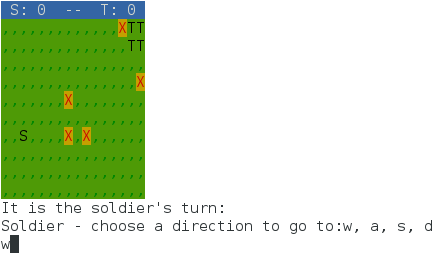
\includegraphics[scale=0.6]{screenshots/terminal003.png}
\caption{The terminal implementation (\texttt{sc\_land}) of the game.}
\label{fig:terminal-screenshot-0}
\end{figure}


By implementing a terminal version, we could test the implementation
much faster and debug with the "GNU Debugger" available, which provides 
much better debugging support than the STK1000 board does. From the
implementaion, we found and solved bugs in regards to correctly placing
scorched land tiles from a bullet shot. We also found out that we forgot to
flip the x-position, and implemented the code needed to flip it.

\subsection{Implementing the user interface}

With all the low level support functions in place, as well as the game
logic itself, a user interface tying all this together was needed. The
user interface is implemented in the files \texttt{ui.c} and
\texttt{ui.h}.

The user interface is a state machine that changes between the following
states:

\begin{enumerate}
    \item Intro screen.
    \item Gameplay, soldier's turn to move.
    \item Gameplay, tank's turn to select shooting angle.
    \item Gameplay, tank's turn to select shooting strength.
    \item Game over screen.
\end{enumerate}

The user interface runs in an infinite loop, rendering to the screen,
reading input, controlling the sound and updating the game state.
